\documentclass{article}
\usepackage[utf8]{inputenc}
\usepackage[spanish]{babel}
\usepackage{listings}
\usepackage{graphicx}

\usepackage{hyperref}
\urlstyle{same}

\graphicspath{ {images/} }
\usepackage{cite}

\begin{document}

\begin{titlepage}
    \begin{center}
        \vspace*{1cm}

        \Huge
        \textbf{Idea Inicial}
            
        \vspace{0.5cm}
        \LARGE
            
        \vspace{1.5cm}
            
        \textbf{Danier Santiago Ortega Restrepo}\\
        \textbf{c.c.1036681098}\\
        
        \textbf{Jose Manuel Rivera Villa}\\
        \textbf{c.c.1000860503}
            
        \vfill
            
        \vspace{0.8cm}
            
        \Large
        Despartamento de Ingeniería Electrónica y Telecomunicaciones\\
        Universidad de Antioquia\\
        Medellín\\
       Octubre de 2021

    \end{center}
\end{titlepage}

\tableofcontents
\newpage
\section{Ideas Iniciales}\label{Ideas}
Nombre del juego: ChangeSpace \newline Espacio: Cuadrícula de M*N (por el momento se tiene pensado 2 filas por 3 columnas) \newline Vista: Tipo plataforma 2D \newline Animación: Pixel art \newline Dinámica: La dinámica principal del mismo es la música. Cada nivel tendrá como espacio jugable un escenario fijo de plataformas el cual se dividira en zonas de tal forma que quede como una cuadricula MxN.  El jugador será situado en la parte inferior izquierda. Luego, cada cierto tempo, he aquí la importancia de la música, se iluminarán un número x de zonas, advirtiendo al jugador que deberá evitar a toda costa las mismas. El objetivo será que el jugador se mueva de espacio en espacio, evitando estar situado en un espacio iluminado, pues tras un corto periodo de tiempo estos espacios se tornarán de un color sólido. Si el jugador se encuentra sobre alguno de ellos perdera la partida y tendra que iniciar de nuevo. La posición de los espacios sombreados se generará aleatoriamente y será al ritmo de la música que estará sonando. La dificultad estará dada por la cantidad x de zonas que se iluminarán con respecto a la cuadricula M*N, y la velocidad en la que se generen, nuevamente se resalta la importancia de la música. El jugador ganara puntos a medida que pase más tiempo sin perder, y el nivel se considerará completo una vez termine la canción. \newline Se planea incorporar distintas canciones con diferente tempo para adecuar la dificultad de cada nivel, en los cuales le corresponderá un distinto tamaño de cuadrícula de ser necesario asi mismo a cantidad de zonas a iluminar.

Según el avance del proyecto se planea tambien agregar proyectiles que serán lanzados desde los laterales del escenario en zonas aleatorias ademas de rocas que caeran de la parte superior, para asi añadir mas dificultad al juego.



\section{Representacion grafica}\label{Video}
\begin{figure}[h]
    \centering
    \caption{Escenario inicial}
    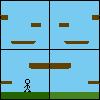
\includegraphics{sprite_0.png}
    \label{fig:my_label}
\end{figure}

\begin{figure}[h]
    \centering
    \caption{Escenario con zonas iluminadas}
    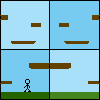
\includegraphics{sprite_1.png}
    \label{fig:my_label}
\end{figure}

\begin{figure}[h]
    \centering
    \caption{Escenario con las zonas de peligro}
    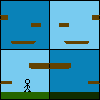
\includegraphics{sprite_2.png}
    \label{fig:my_label}
\end{figure}

\begin{figure}[h]
    \centering
    \caption{Cabio de zonas iluminadas}
    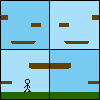
\includegraphics{sprite_3.png}
    \label{fig:my_label}
\end{figure}

\begin{figure}[h]
    \centering
    \caption{Movimiento del jugador}
    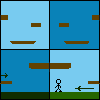
\includegraphics{sprite_4.png}
    \label{fig:my_label}
\end{figure}

\bibliographystyle{IEEEtran}


\end{document}